\documentclass[letterpaper, 12pt]{article}
\raggedbottom{}
\usepackage[utf8]{inputenc}
% \usepackage[papersize={216mm,330mm},tmargin=15mm,bmargin=15mm,lmargin=15mm,rmargin=15mm]{geometry}
\usepackage[english, spanish]{babel}
\usepackage{fullpage} % changes the margin
\usepackage{graphicx}
\usepackage{enumitem}
\usepackage{chngcntr}
\usepackage{multirow}
\usepackage{parskip}
\usepackage{url}
\usepackage{booktabs} 
\counterwithin{figure}{section}
\renewcommand{\thesection}{\arabic{section}}
\renewcommand{\thesubsection}{\thesection.\arabic{subsection}}
\renewcommand{\baselinestretch}{1.5}
\usepackage{float}
\usepackage{apacite}
\usepackage{multicol}
\setlength{\columnsep}{.4cm}
\bibliographystyle{apacite}
\setlength\belowcaptionskip{10pt}
\linespread{1.5}

\begin{document}

% PRACTICA 5
%  GUÍA No. 7

\begin{titlepage}
	\centering
	
\includegraphics[width=0.3\textwidth]{Images/logo_utb.png}\par\vspace{1cm}
	{\scshape\LARGE Universidad Tecnológica de Bolívar \par}
	\vspace{1cm}

	{\scshape\Large FÍSICA ELÉCTRICA \par}
	\vspace{.2cm}

	% chktex-file 8
	{\scshape\Large H1 - C \par}
	\vspace{1cm}
	% chktex-file 8 chktex-file 13
	\slshape {\Large \bfseries{} LAB 5 - CAMPO MAGNÉTICO EN UNA BOBINA. FUERZA MAGNÉTICA\\}
	\slshape {\small \bfseries{} Guía de laboratorio No. 7}
	\vspace{1cm}

	\slshape {\itshape{} Mauro González, T00067622 \\}
	\slshape {\itshape{} German De Armas Castaño, T00068765 \\}
	\slshape {\itshape{} Angel Vega Rodriguez, T00068186 \\}
	\slshape {\itshape{} Juan Jose Osorio Ariza, T00067316 \\}
	\slshape {\itshape{} Juan Eduardo barón, T00065901 \\}
	\vfill
	Revisado Por \\
	Gabriel Hoyos Gomez Casseres\\
	{\large \today\par}
\end{titlepage}

% ----------------------------------------------------------------------|>
\begin{multicols}{2}

\section{Introducción}


% ----------------------------------------------------------------------|>
\section{Objetivos}

\subsection{Objetivos Generales}


% ----------------------------------------------------------------------|>
\section{Preparación de la practica}

% -----------------------------------------------------------|>
\subsection*{Calcula el campo magnético sobre el eje de un solenoide y llega a la expresión (1).}

El objetivo es calcular el campo eléctrico de un solenoide en un punto P situado
en el eje del solenoide sumando el campo producido por las N espiras.

\begin{figure}[H]
	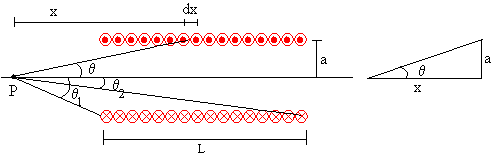
\includegraphics[width = \linewidth]{./Images/solenoide.png}
\end{figure}

En la figura, tenemos un corte longitudinal de un solenoide de longitud L,
formado por N espiras iguales de radio a.

De~\cite{CampoElectricoPorEspira} se obtuvo la expresión para calcular el campo
magnético producido por una espira de radio $a$ en un punto $P$ de su eje
distante $X$.

	% chktex-file 3
	{\large $B = \displaystyle\frac{\mu_0 i a^2}{2 \left(\sqrt{a^2 + x^2}\right)^3}$}

Todas las espiras del solenoide producen sobre P un campo que tiene la misma
dirección y sentido, pero distinto módulo, dependiendo de la distancia $X$ al
punto P.

El número de espiras que hay en el intervalo comprendido entre
$x$ y $x+dx$ es $dn = N \cdot \frac{dx}{L}$

Estas espiras producen en P un capo que es el producto del campo producido por
una espira por el numero de espiras.

	{\large $dB = \frac{\mu_0 i a^2}{2 \left(\sqrt{a^2 + x^2}\right)^3} \cdot \frac{N}{L} dX$}

Para integrar, tenemos que hacer el cambio de variable $a = \tan\theta$ y
teniendo en cuenta que, {\large $1 + \tan^{2}\theta = \frac{1}{\cos^{2}\theta}$},
simplificamos la integral

	{\large $B = \frac{\mu_0 i N}{2L} \int_{\theta_1}^{\theta_2} -\sin\theta \cdot \,d\theta$}

	{\large $ = \frac{\mu_0 i N}{2L} \left(\cos\theta_2 - \cos\theta_1\right)$}

Si el solenoide es muy largo comparado con su radio $a$ y si el punto $P$ esta
situado en el centro, tendremos que $\theta_1 \rightarrow \pi$ y
$\theta_2 \rightarrow 0$. El campo $B$ vale entonces:

{\large $B = \frac{\mu_0 i N}{L}$}

Fuente:~\cite{CampoElectricoSolenoide}

% -----------------------------------------------------------|>
\subsection*{Demuestra la expresión (3) y (4) realizando los esquemas necesarios para las corrientes, el
	campo y la fuerza resultante}

% ----------------------------------------------------------------------|>
\section{Resumen del procedimiento}

\end{multicols}

\newpage

\bibliography{./Bibliography/bibliography.bib}

\end{document}